\newcommand{\agentsegments}{256}\newcommand{\agenteta}{47.0}\newcommand{\agentetafar}{20.2}\newcommand{\agentfarpct}{7.9}\newcommand{\agentring}{5--15}
\subsection*{The agent's run}
Request: \emph{Focus the beam.} --- nothing else was typed. Model: \texttt{claude-cli:claude-sonnet-5-5}.

\begin{longtable}{@{}r r r r c r r r c r r@{}}
\toprule exp & macropixel & segments & focus & ring $r$ [px] & regions & iterations & flips & remeasure & $\eta$ & $\eta_\text{far}$\\\midrule\endhead
1 & 8 & 64 & 3 & 5--15 & 8 & 20000 & 4$\to$1 & yes & 9.8$\pm$0.1 & 7.6\\
\rowcolor{yellow!25}2 & 4 & 256 & 3 & 5--15 & 8 & 40000 & 8$\to$1 & yes & 47.0$\pm$0.1 & 20.2\\
3 & 16 & 16 & 3 & 5--15 & 8 & 10000 & 2$\to$1 & yes & 2.7$\pm$0.1 & 2.6\\
\bottomrule
\end{longtable}
Kept by the agent: experiment 2, enhancement 47.0 (far field 20.2). Diagnostics only the simulation knows: noise-free 47.3, known-$T$ binary pattern 25.7 (far field), theory $N_\text{eff}/2\pi=19.6$.
\begin{figure}[H]\centering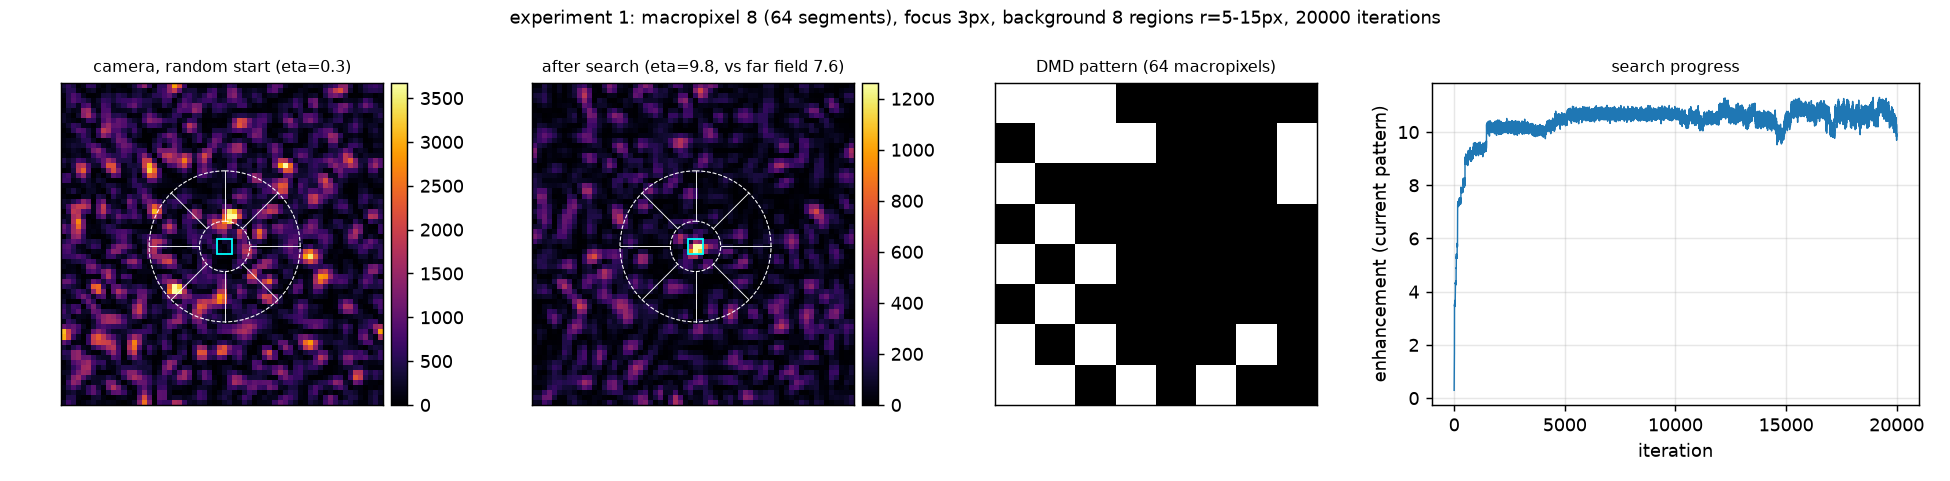
\includegraphics[width=\linewidth]{hw2_figs/agent_run/experiment_01.png}\caption{Agent experiment 1.}\end{figure}
\begin{figure}[H]\centering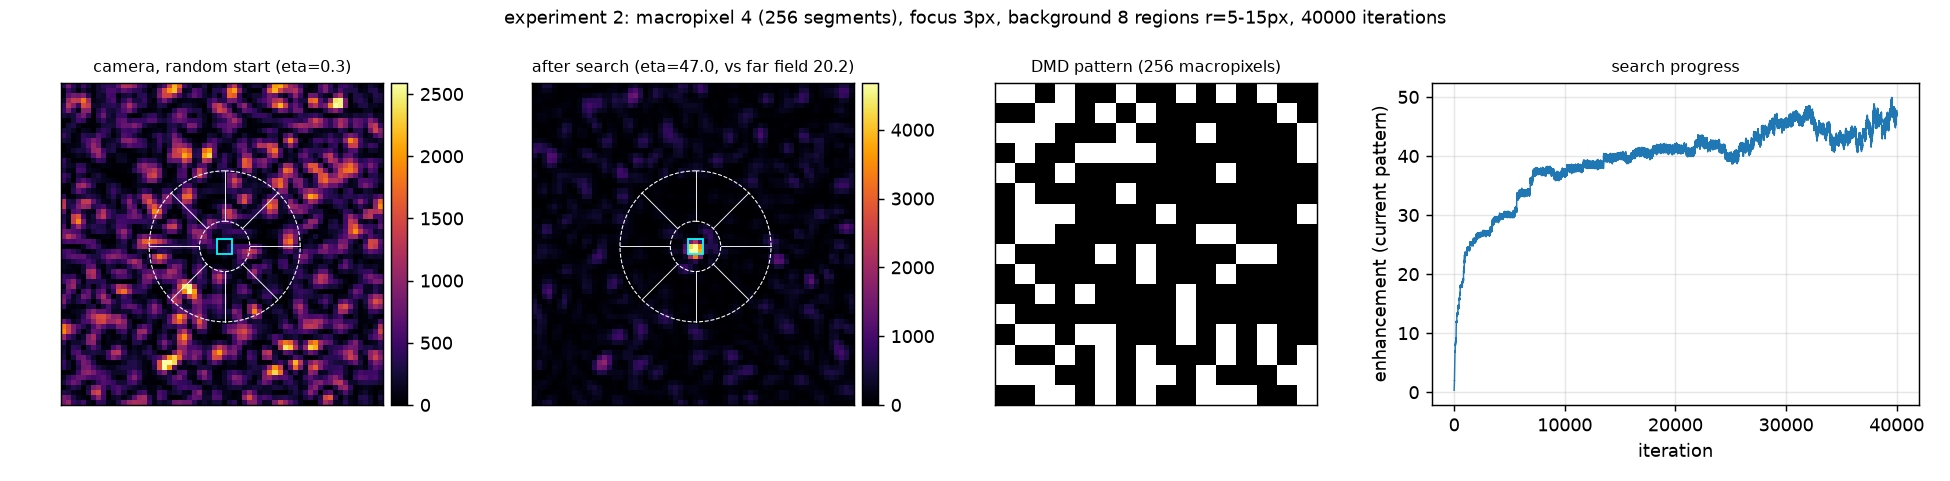
\includegraphics[width=\linewidth]{hw2_figs/agent_run/experiment_02.png}\caption{Agent experiment 2.}\end{figure}
\begin{figure}[H]\centering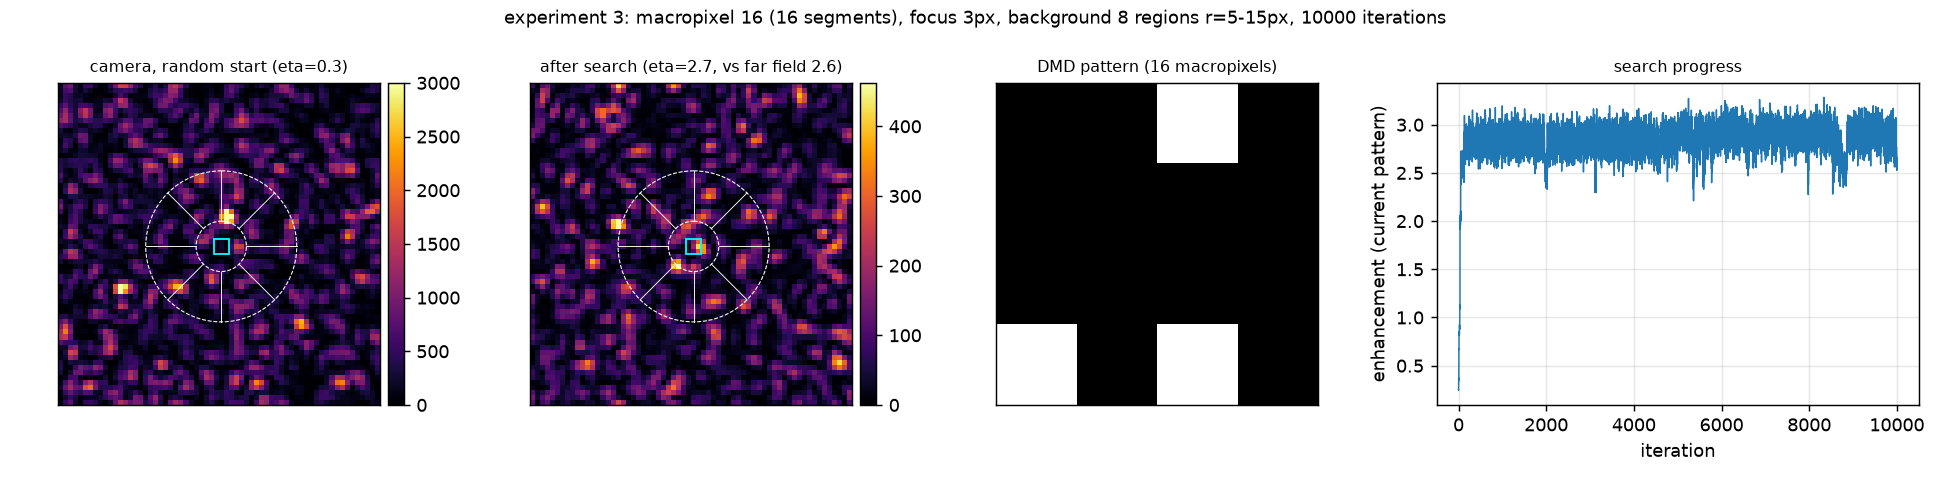
\includegraphics[width=\linewidth]{hw2_figs/agent_run/experiment_03.png}\caption{Agent experiment 3.}\end{figure}
\paragraph{Who did what.}
\begin{longtable}{@{}r l p{0.74\linewidth}@{}}
\toprule \# & role & what it did\\ \midrule \endhead
1 & user & Focus the beam.\\
2 & orchestrator & -\textgreater{} scientist: No plan exists yet, so the scientist must define the focusing procedure before the executor can run it.\\
3 & scientist & \# Plan: focus the beam with `focusing\_tool` The standing brief asks for an ODE and neural-network plan with a voltage RMSE test. The instruction in this turn is a beam...\\
4 & orchestrator & -\textgreater{} executor: A plan now exists and only the executor can run the tools to produce a verified measurement.\\
5 & executor & experiment 1: \{"macropixel": 8, "focus\_size": 3, "bg\_inner": 5, "bg\_outer": 15, "bg\_regions": 8, "iterations": 20000, "flips": 4, "flips\_final": 1, "remeasure": true, ...\\
6 & orchestrator & -\textgreater{} finish: A VERIFIED measurement exists and the budget is limited, so I'll report the results to the user.\\
\bottomrule
\end{longtable}
